\documentclass[10pt, conference, a4paper]{IEEEtran}
\usepackage{cite}
\usepackage[dvips]{graphicx}
\usepackage[tight,footnotesize]{subfigure}
%\usepackage{flushend}
\hyphenation{op-tical net-works semi-conduc-tor}


\begin{document}
\title{Research and Implementation of an IMS-based AS/MRFC Model for IVR Services}


\author{\IEEEauthorblockN{Youzheng Chen, Baozhong Cheng, and Xiaoyan Zhang}
\IEEEauthorblockA{School of Software Engineering\\
Beijing University of Posts and Telecommunications\\
Beijing, China\\
Mr.Youzheng.Chen@ieee.org\\
bzcheng@bupt.edu.cn}
}

\maketitle


\begin{abstract}
IVR is well known for being able to facilitate interaction between user and computer system. Integrated into IMS service platform, IVR applications can provide value-added services for IMS subscribers. According to the survey of current situation on IVR systems, this research mainly proposes a more flexible and scalable solution on IMS-based AS/MRFC model for IVR services by providing efficient business adaptation. Deployed on JAIN SLEE, this solution can work with MRFP to provide IVR services to IMS users. Finally, the proof of the feasibility and compatibility of this solution is presented, which also shows its broad prospects among some application scenarios. This paper discusses problem analysis, architecture design, application implementation and system evaluation of this solution.

\end{abstract}

\begin{IEEEkeywords}
IMS; AS; MRFC; JAIN SLEE; IVR; MRCPv2; VoiceXML

\end{IEEEkeywords}

\IEEEpeerreviewmaketitle

\section{Introduction}
Proposed by the Third Generation Partnership Project (3GPP), Internet Protocol Multimedia Subsystem (IMS) is a service development architecture for the Next Generation Network (NGN)\cite{standard:3gpp.23.228}. Interactive Voice Response (IVR) is one of the important techniques to develop new self-services in IMS network for reducing IMS running cost. However, most of the IVR systems nowadays are designed for a small scale, so they may not be scalable and flexible enough for the requirement of IMS network. Thus, a prototype application of Application Server (AS) / Media Resource Function Controller (MRFC) model for controlling Media Resource Function Processor (MRFP) is developed for the purpose of providing IVR services to IMS Users. 

In this research work, a new solution of IVR Function in IMS area is proposed. In the meantime, the current IMS network elements can be seamless to support this function. The main contributions of this research are:
\begin{itemize}
\item Propose an architecture of value-added business with high scalability and openness for business adaptation;
\item Develop and implement a prototype to prove the feasibility and compatibility of this solution;
\item Evaluate the proposed solution and provide some application scenarios.
\end{itemize}

This paper mainly presents a research about IVR Function in IMS network, and especially describes the development of AS/MRFC model in this function, which provides a prototype application for further research on IVR Function Controller.

\section{Problem Analysis}

As speech recognition technology making a great progress in recent years, IVR technology has been applied into more and more areas to reduce running cost and improve user experience. In the near future, IVR services will play an important role in our daily life.

\begin{figure}[!t]
\centering
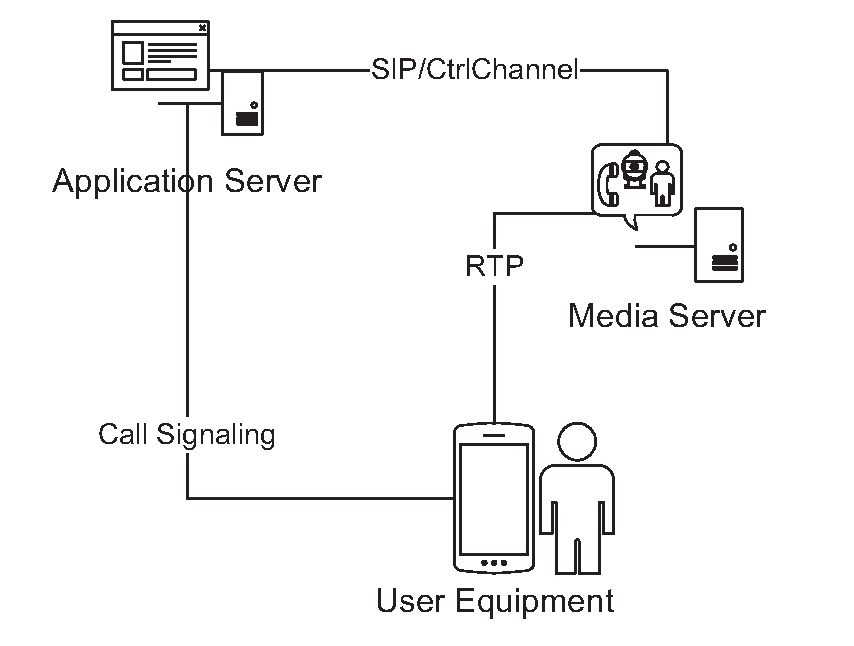
\includegraphics[width=2.7in]{ivr_topology.eps}
\caption{Traditional Topology of IVR Services.}
\end{figure}

Figure 1 shows a traditional topology of IVR services, which is proposed in RFC 5567\cite{misc:rfc5567}. This architecture depicts the basic IVR services, which involve an Application Server (AS) and a Media Server (MS). The AS establish the media control channel via Session Initiation Protocol (SIP) and manipulates the MS via this channel in order to provide specific services to their users. However, this architecture may not be suitable for complex requirement of IMS, even if a higher level of abstraction have been applied to some advanced IVR services for describing business logic, for example, using one or more back-end servers to host Voice eXtensible Markup Language (VoiceXML)\cite{misc:voice.extensible.markup.language} documents.

\begin{figure}[!t]
\centering
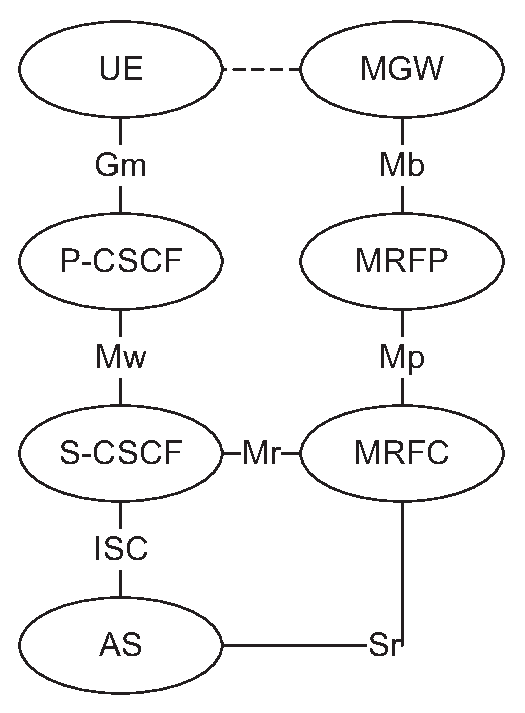
\includegraphics[width=1.5in]{standard.eps}
\caption{The 3GPP Architecture of MRF.}
\end{figure}

The 3GPP standard architecture of Media Resource Function (MRF) is shown in Figure 2. AS is an entity that deals with the main business logic and controls the related network elements to provide services for subscribers. MRFC is an entity that is used to control MRFP for the handle of media resources. 

In order to integrate IVR system into IMS network as a value-added service, the architecture of IMS defined by 3GPP is referred and improved for the specific requirement in this area. For the requirement of providing separated services to different subscribers, the user preferences should be recorded in this system. These user preferences are named as Subscriber Policy in this paper. Using Subscriber Policy Server, we can retrieve the specific preference when a call is incoming. In addition, the higher level of abstraction, which is used to describe the business logic, is named Speech Script in this paper. The back-end server, which provides the specific Speech Script, is named Speech Script Server. The script it provides can be static, which is stored in file system, or it can also be dynamic. In the second case, the script can be dynamically generated as JavaServer Pages (JSP) or Servlet according to the business logic and the user preferences.

In the recommendation of 3GPP, it is not clear about different roles between AS and MRFC in IVR Function. In one way, we can combine the function of AS and MRFC, which is formed a collocated AS/MRFC model, so that it is capable of playing the role of configuring and managing the business logic. However, this is a tightly coupled model, in which case this IVR Application acts as a SIP user agent to communicate with all the subscribers, and all the processes of business logic will be finished internally, which makes the topological graph like a centralized star. It is not a good design for the complex requirement of IMS.

\section{Architecture Design}

In order to solve this problem, we have consulted the Technical Report of 3GPP\cite{standard:3gpp.24.880}. It has proposed a solution for functional split between the AS and MRFC on conference focus. Such solution can also be applied to our situation with necessary modifications. In this way, we propose our solution of IVR Function (shown in Figure 3). The terminology and concepts are still reused from the Internet Engineering Task Force (IETF) standards and the definition described above.

\begin{figure}[!t]
\centering
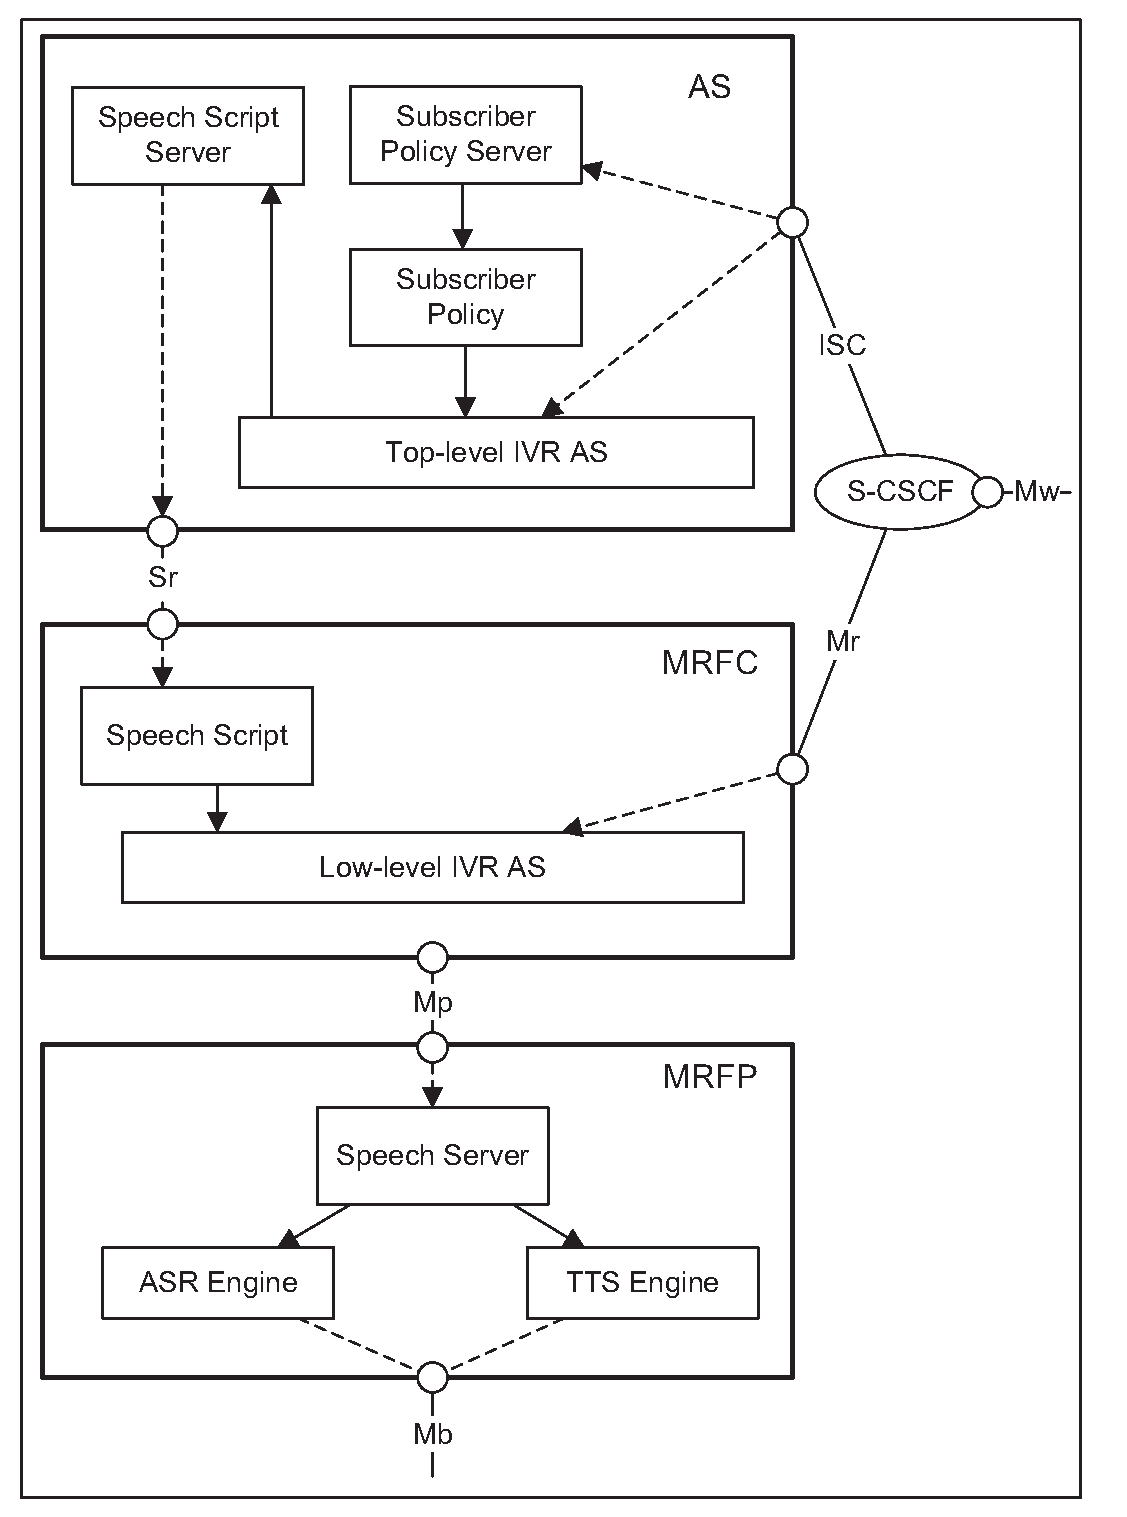
\includegraphics[width=3.3in]{split.eps}
\caption{Our Solution of IVR Function.}
\end{figure}

The collocated AS/MRFC model is split between two sets of servers: Top-level IVR AS and Low-level IVR AS. The Top-level IVR AS, which maintains the role of IMS AS, is used to handle the jobs related to the preferences of subscribers, while the Low-level IVR AS, which plays the role of IMS MRFC, is used to deal with the speech application logic assigned by the top-level ones.

In details, the Top-level IVR AS, is used to
\begin{itemize}
\item Implement the Subscriber Policy Server, for identifying the incoming call and present the related user preference. And the user data can be subscribed and modified by the end-users.
\item Generate the related business logic through Speech Script Server accordingly and send to the Low-level IVR AS.
\item Maintain user dialogs and redirect or transfer dialogs according to the instruction of the Low-level IVR AS.
\item Might support billing and charging.
\end{itemize}

And the Low-level IVR AS, is used to
\begin{itemize}
\item Load and execute the Speech Script, such as VoiceXML\cite{misc:voice.extensible.markup.language}, CCXML\cite{misc:voice.browser.call.control}, and SCXML\cite{misc:state.chart.xml}.
\item Control the speech-related logic on MRFP, and the dialog manipulation on AS.
\end{itemize}

To consider about the programming model between the Top-level and the Low-level IVR AS, we can't ignore the two major models, which are popular among software design: delegation model and protocol model. The delegation model is a coarse-grained model, which holds the communication between two sides through transferring Extensible Markup Language (XML) scripts, while the protocol model is a fine-grained model, which utilizes dedicated channel to transfer data via specific protocol. For the reason of the type and size of Speech Script, the delegation model is applied to the communication between AS and MRFC. Using Sr interface, the Speech Script can be transmitted via Hypertext Transfer Protocol (HTTP). In addition, the data between MRFC and MRFP is trivial but needed to be transferred orderly. So instead of using SIP protocol over User Datagram Protocol (UDP), we prefer to create a dedicated channel via Mp interface to prove the stability of data transfer.

To specify an independent protocol for the control of MRFP by MRFC on IVR Function via Mp interface, we should consider the correlation of business logic, including speech synthesis, speech recognition, Dual-Tone Multi-Frequency (DTMF) recognition, and speaker verification. The main requirement of this protocol is to help MRFC to send discrete IVR instructions to MRFP. In this research, we have tried to:

\begin{itemize}
\item use Media Gateway Control Protocol (MGCP)\cite{misc:rfc3435}, which is used for signal transmission between AS and media server (MS), but with few definitions on Speech Recognition;
\item use Media Resource Control Protocol (MRCP)\cite{misc:rfc4463}, to transmit signals between application server and speech server, which has a complete definition on Speech Synthesis and Speech Recognition, but it transmits over Real Time Streaming Protocol (RTSP), which may interfere with the normal media stream control;
\item use Media Resource Control Protocol Version 2 (MRCPv2)\cite{misc:rfc6787}, which is used for transmitting data through channels created by SIP and Session Description Protocol (SDP).
\end{itemize}

In this scenario, in terms of the ability of information expression on speech and the interference of control signal and media stream, MRCPv2 is considered to be the best choice of transport protocol in this solution.

\section{Implementation}

\begin{figure}[!t]
\centering
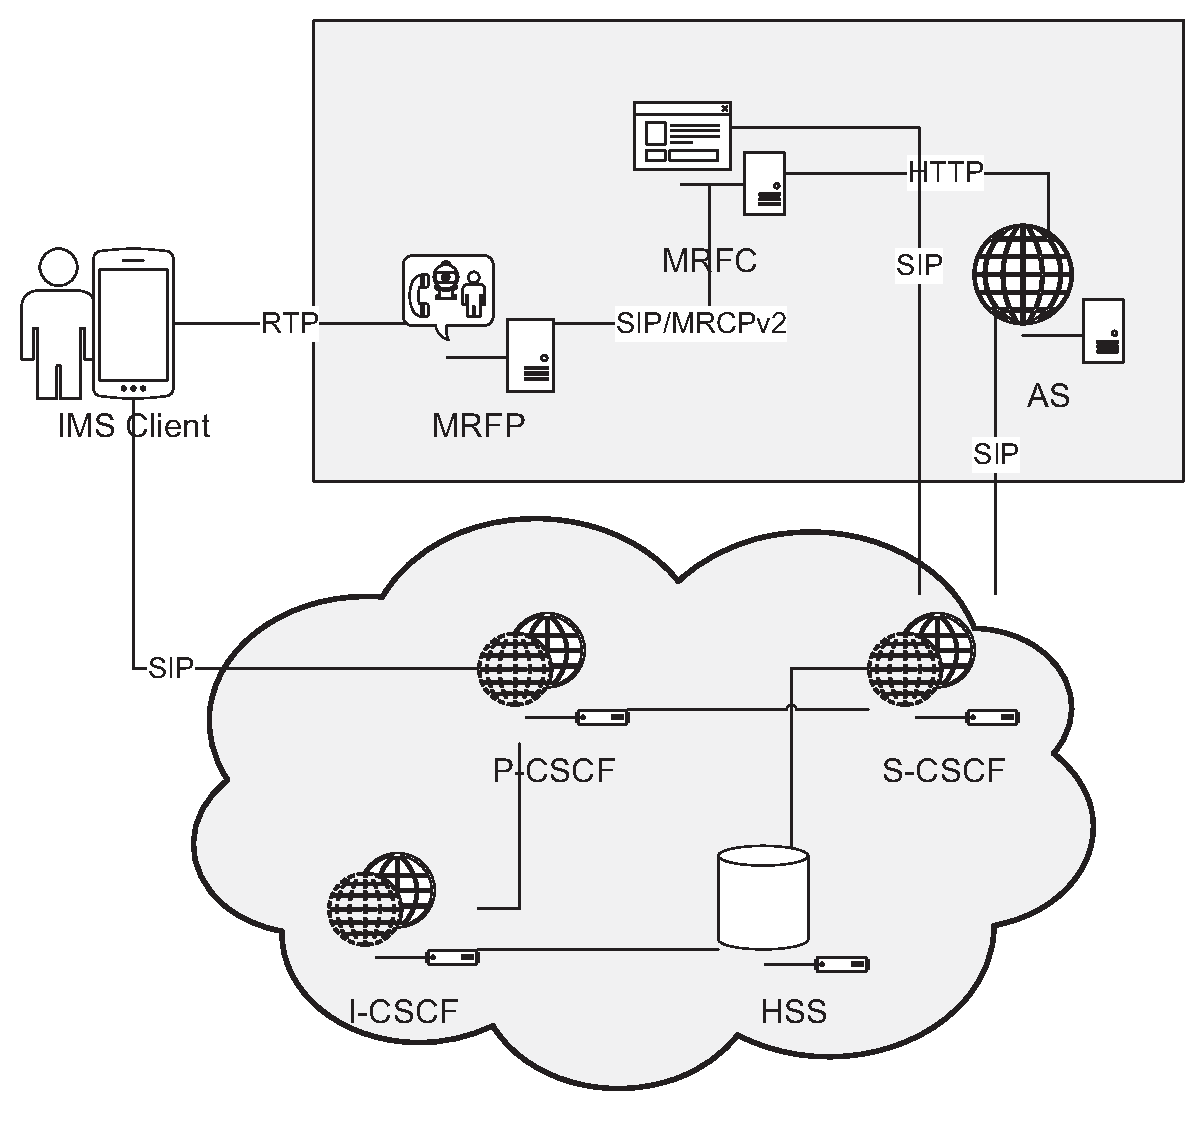
\includegraphics[width=3.1in]{architecture.eps}
\caption{The Architecture of the Solution.}
\end{figure}

According to the design described above, a prototype project is designed and implemented in order to prove the feasibility. As Figure 4 depicts, this solution can be viewed as three parts: IMS Client, IMS Core and IMS Services.

Here, IMS Client plays a role of the User Agent Client (UAC) that presents user interface (UI) to client actor and deals with the client logic for IMS network. 

IMS Core is a function that is used for handling signal switch and call control. In this system, IMS Core contains four main network elements: Proxy-Call Session Control Function (P-CSCF), Interrogating-CSCF (I-CSCF), Serving-CSCF (S-CSCF) and Home Subscriber Server (HSS)\cite{book:softswitch.and.ims.technology}. IMS Core communicates with other network elements in this solution via SIP Protocol.

IMS Services in this scenario has only one function - providing custom IVR services. According to user preference, AS presents specific script of business logic to MRFC via HTTP protocol. MRFC parses scripts and controls MRFP via MRCPv2 protocol to finish speech-related jobs by providing custom services to the specific subscriber.

\begin{figure}[!t]
\centering
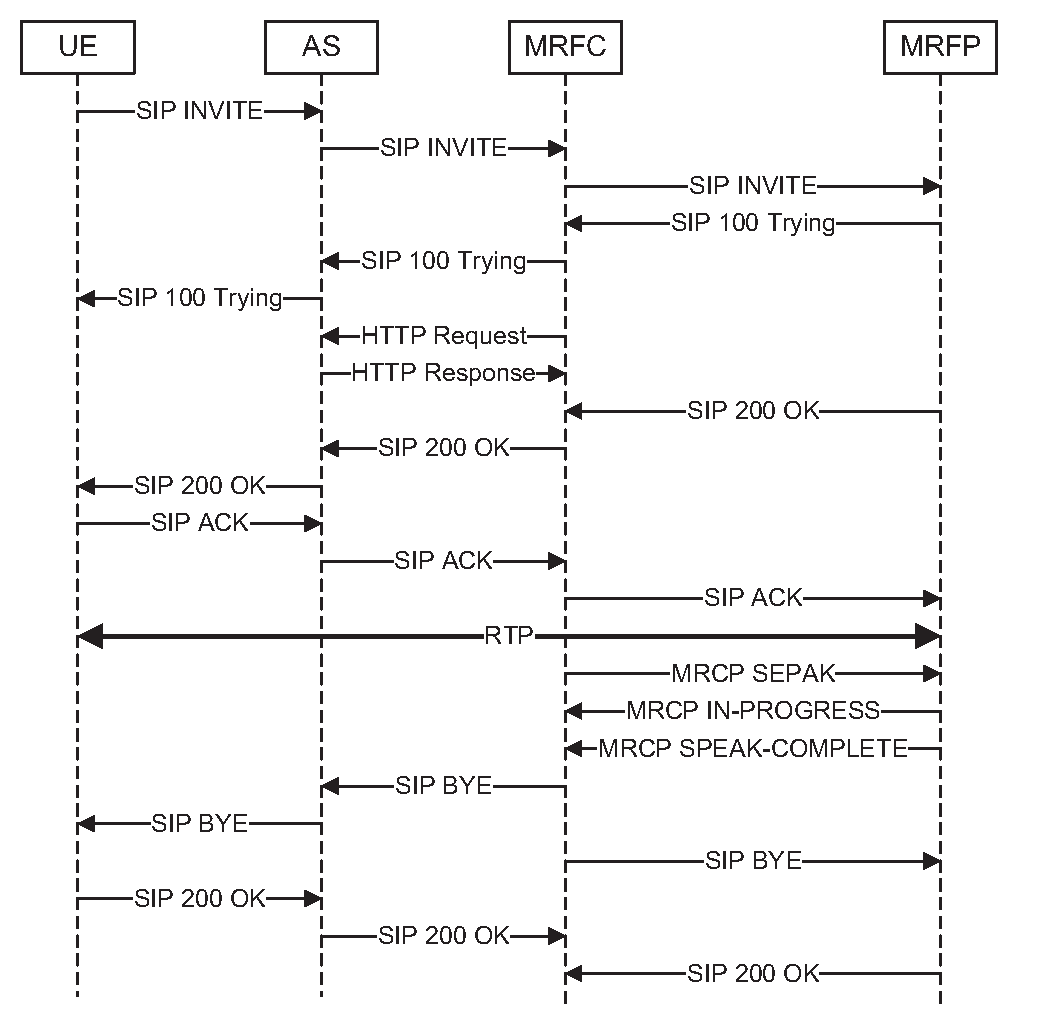
\includegraphics[width=3.3in]{callflow.eps}
\caption{The Call Flow of a Basic Scenario.}
\end{figure}

The call flow (shown in Figure 5) depicts the basic scenario of our solution. Assuming that there is a subscriber utilizing the User Equipment (UE) to send a SIP INVITE message via IMS Core (not shown in the figure) to AS. AS retrieves the user preference, which stored in its database and forwards this message to MRFC with necessary user preference. According to user preference (e.g. this user may prefer to use DTMF instead of Speech), MRFC sends SIP request to MRFP in order to open related dedicated channel. In addition, MRFC sends HTTP request to AS for the purpose of retrieving specific scripts of business logic. When the media channel is established, the MRFC sends MRCP request to control MRFP finish application logic. What's more, when meeting with the call control operations, MRFC will request AS to finish related instructions.

In this solution, the design of IMS core network is out of our scope. We will only focus on the portion of media resource control, including AS and MRFC. For the purpose of facilitating the rapid development of this prototype project, we use Java as main development language. Since SIP Servlet is incapable of providing a well-defined mechanism to extend protocol support, Java APIs for Integrated Networks Service Logic Execution Environment (JAIN SLEE) technology\cite{standard:jslee.v11.specification} is adopted as the container instead of SIP Servlet technology, to host the applications, which provide the function of AS/MRFC. This efficiently helps us focus on business logic development instead of concurrency control or failure model. And JAIN SLEE technology can completely satisfy the requirement of telecommunication services in service providers rather than SIP Servlet\cite{Chrighton:2007gt}. 

\begin{figure}[!t]
\centering
\subfigure[Processing Flow of AS.]{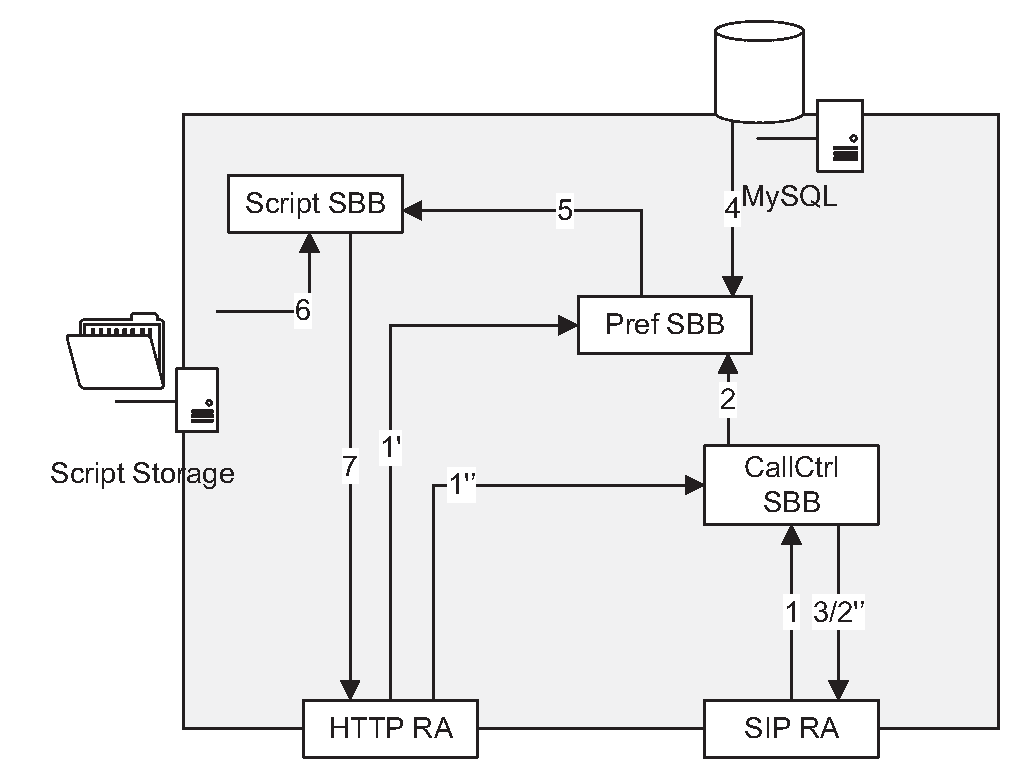
\includegraphics[width=3in]{implementation_a.eps}}
\subfigure[Processing Flow of MRFC.]{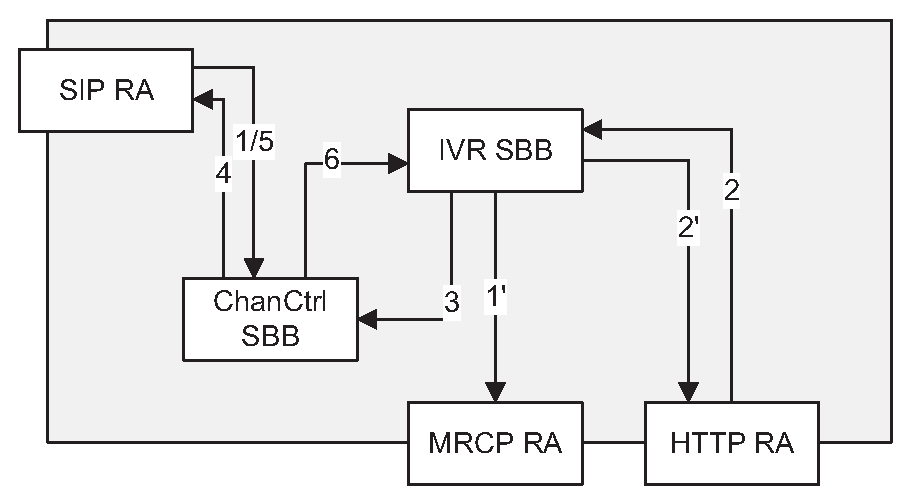
\includegraphics[width=3in]{implementation_b.eps}}
\caption{The Functional Entities and Processing Flow of the Solution.}
\end{figure}

Figure 6 shows the design of functional entities in our solution. This design can be divided into two parts: AS and MRFC. As Subfigure (a) depicts, The AS mainly implements the function of retrieving scripts of business logic depending on user preferences. The Sr interface and ISC interface require the communication via HTTP protocol and SIP protocol, so we added two JAIN SLEE Resource Adaptor (RA): HTTP RA and SIP RA. And we designed three main Service Building Blocks (SBBs) to implement the business logic of AS: Pref SBB, Script SBB and CallCtrl SBB. First, When a SIP call is incoming (1), CallCtrl SBB will identify the message and forward it to Pref SBB (2). Then this message will also be forwarded to specific MRFC via SIP RA (3). Pref SBB plays a role of Subscriber Policy Server, which can identify users from incoming dialog and retrieve user data from MySQL database (4). Then it will provide essential user preference to Script SBB (5). Script SBB acts as Speech Script Server, which can statically retrieve scripts from file system or dynamically generate scripts for specific requirement (6), and present the scripts as VoiceXML documents via HTTP RA (7). Second, The user preferences can be configured or managed by XML Configuration Access Protocol (XCAP) Client via HTTP RA (1'). Third, when MRFC sends the control signals via HTTP protocol, CallCtrl SBB can receive that event (1'') and then use SIP RA to manipulate the dialogs (2'').

Subfigure (b) shows that the MRFC plays a role of media controller according to the script sent by AS. When the call forwarded by AS is incoming, ChanCtrl SBB is used to received this event via SIP RA (1). When the user preference is arrived, IVR SBB is used to handle this event (2) and tell ChanCtrl SBB the specific requirement of the user (3). Accordingly, ChanCtrl SBB constructs essential session description for creating dedicated channel of MRCPv2 protocol and sends the modified INVITE message to MRFP via SIP RA. After MRFP confirms and sends back the MRCPv2 channel message (5), ChanCtrl SBB will forward the information to IVR SBB. By parsing the scripts of application logic, IVR SBB controls MRFP via MRCP RA (1'). And if involving dialog manipulation, IVR SBB will inform AS via HTTP RA (2').

\section{Test and Discussion}

The purpose of testing this solution is to ensure the interoperability with other IMS network elements. This test utilizes some Open Source Projects that fit for this architecture. The architecture of this test case is divided into four separate parts: IMS Client, IMS Core, IMS AS and IMS MRFC/MRFP. In IMS Client part, we use iDoubs designed by Doubango Telecom\cite{site:doubango}, which is run on Mac OS system. In IMS Core part, we use Open IMS Core designed by Fraunhofer FOKUS\cite{site:open.ims.core}. In IMS MRFP part, we use UniMRCP\cite{site:unimrcp} as Speech Server. In IMS AS/MRFC part, we use Mobicents JAIN SLEE\cite{site:mobicents.jain.slee} as the container and deploy our solution on it. These parts are run in Ubuntu system. The entire architecture is shown in Figure 7.

\begin{figure}[!t]
\centering
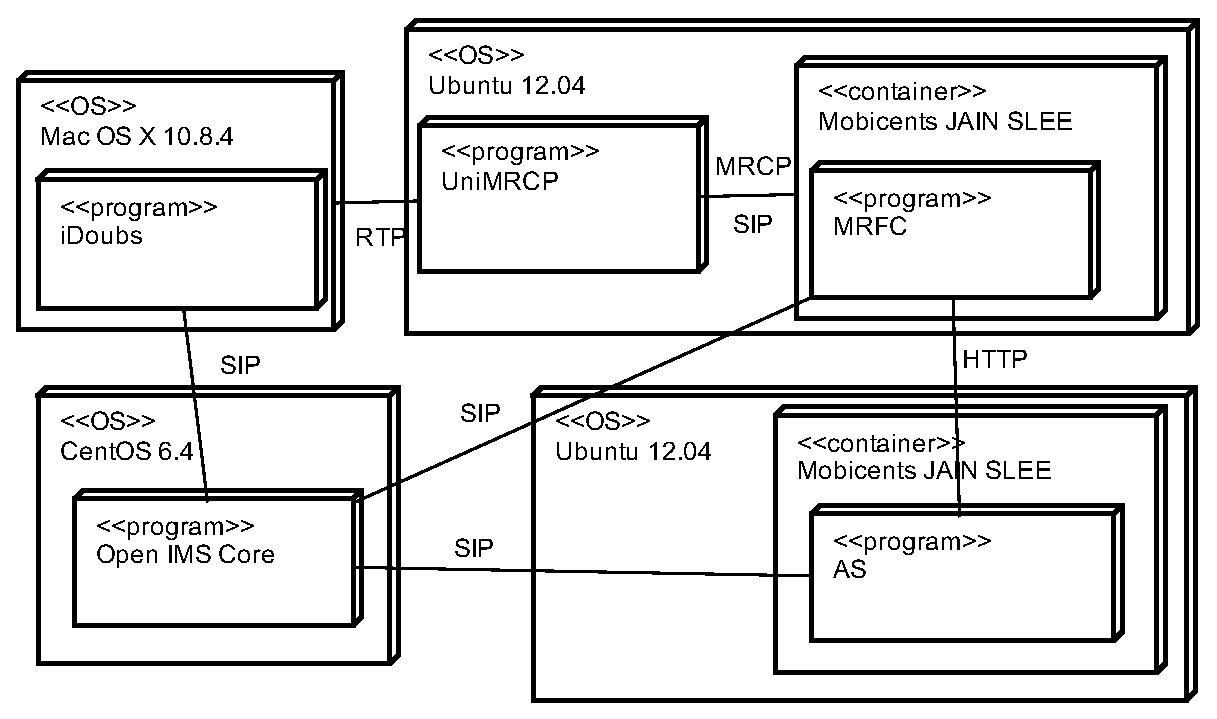
\includegraphics[width=3.1in]{deployment.eps}
\caption{The Deployment Diagram of Our Solution.}
\end{figure}

In this scenario, we simulate a classic runtime environment for the Media Resource Function. To evaluate the feasibility of our solution, we design a process for testing. First, we use IMS Client to register in IMS Core. After registration successful, we use IMS Client, which is preset for the subscription of the user, to send a Voice Call. After the AS generates specific VoiceXML documents according to user preference, MRFC builds up the dedicated channel with MRFP, then the RTP connection between IMS Client and MRFP is connected. We have test speech recognition, DTMF recognition, speech synthesis and the hybrid of the three using custom user preferences. After that, when IMS Client send BYE message, the allocated resource is released normally. 

\begin{figure}[!t]
\centering
\subfigure[User Preference Shared by Different Services.]{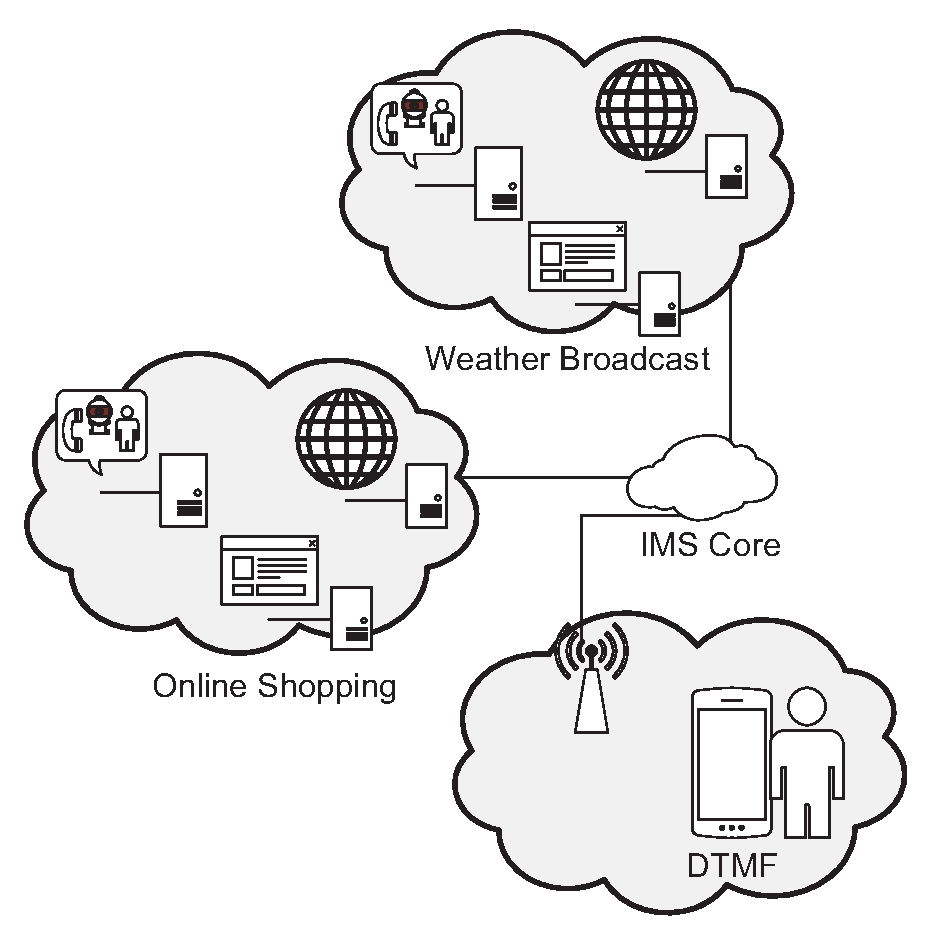
\includegraphics[width=1.6in]{scenario_a.eps}}
\subfigure[Different User Preferences Hosted by the Same Service.]{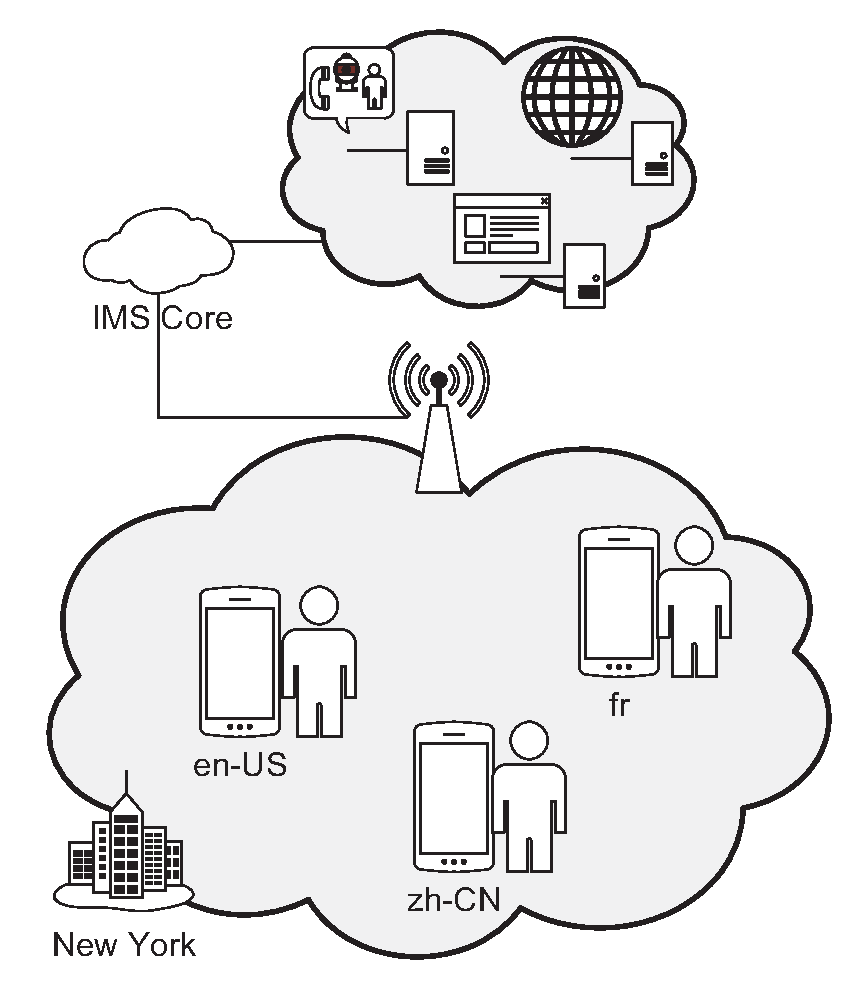
\includegraphics[width=1.6in]{scenario_b.eps}}
\caption{The Application Scenarios.}
\end{figure}

Last but not least, for the application of this solution, we present two scenarios, which significantly show the improvement of the user experience and the reduction of the running costs brought by our solution. Figure 8 depicts two of these application scenarios. Subfigure (a) shows a user who only wants to use DTMF Recognition instead of Speech Recognition. The only thing he has to do is to set his user preference once. And then all the services he subscribed will access the database of Subscriber Policy Server to customize his own scripts of application logic. Subfigure (b) describes that travelers coming from different countries, who want to access the local services, will be always provided in their own language, because the local services can access the user preference from their Home Subscriber Policy Server.

\section{Conclusion}

In this research, the functional split between AS and MRFC in IVR Function provides a new solution to IVR Function in IMS network area, which not only brings telecommunication service providers an opportunity to integrate most of the IVR services through customized speech scripts, but also improves the user experience for subscribers through shared user preference information among different services and different providers.

This paper mainly discusses a prospective architecture solution of IVR Function in IMS area, and provides a development case for IVR Function using JAIN SLEE Technology. In the near future, IVR Technology will be applied to broader areas, such as access control system in apartment, medical call center system and many other areas in the world. In the meantime, IVR Technology is evolving into Interactive Voice and Video Response (IVVR), which is capable of building a video response enhancement system, making it possible for Video on Demand (VOD), Video Sharing, Video Box, which will bring unlimited commercial opportunities for the next-generation value-added business in telecommunication industry.

\section*{Acknowledgment}
The authors would like to thank Kun Li for his valuable advice on architecture design and implementation. And thank Hongye Qi for his contribution to functional requirement.


\bibliographystyle{IEEEtran}
\bibliography{paper}

\end{document}